\subsubsection{Iteration 2: Supporting Learning through UI and Tutorial}

\paragraph{Redesign}

Last iteration, the result shows that the user can not initially understand the controller interaction. A tutorial should be added in this iteration. Also a HUD feedback of the current joystick position is also needed. And a limited collider as a safe piloting environment is also needed.

Interaction Game Objects including the following elements. Quad, DroneVision and Instruct.
The Quad GameObject act as the quadcopter. 

The droneVision GameObject uses Unity's RenderTexture to render the video feed from the quadcopter act as the FPV goggles.

The instruct GameObject shows tutorials for player to learn simple joystick interaction of the quadcopter.

The tutorials including basic controller instructions recorded in video, it is presented in linearly from arm, throttle, yaw, pitch and roll. Each tutorial, the drone Rigidbody will be locked in order to form a \textcite{kolb1984}'s reflective observation. 

For user to clearly aware the joystick position, two cross axis HUD in the view xr reference is added and two dots in the scene shows the current joystick position.

There are 6 interactions the player has to learn, 5 are inclusive of quadcopter's HCI \cref{fig:mode2}. 
Arm, use to start the rotors, is to drag the left stick down to zero.
Throttle, increase or decrease the rotor speed, 
change the longitudinal force of the quadcopter's body, is to turn the left stick up and down.
Yaw, turn the quadcopter's body left and right, is to turn the left stick left and down.
Pitch, control the quadcopter lean forward and back, is to turn the right stick up and down.
Roll, control the quadcopter lean left and right, is to turn the right stick left and right.

The last interaction is to Grip or Select, which is used to click on a button or drag some interactive element.
It uses the grip button on either of the controllers.


The DroneXrEmulator \cref{fig:quad_structure} is added a new parameter to accept an BoxCollider as the safe piloting area.

\paragraph{Enactment}

The refined system keeps the User in an video passthrough environment, but added abstract element that one-to-one mapping with the quadcopter piloting gadgets in reality. 

% Need to change to the latest version
\begin{figure}[H]
    \caption{structure of the interaction elements}\label{fig:interact}
    \centering
    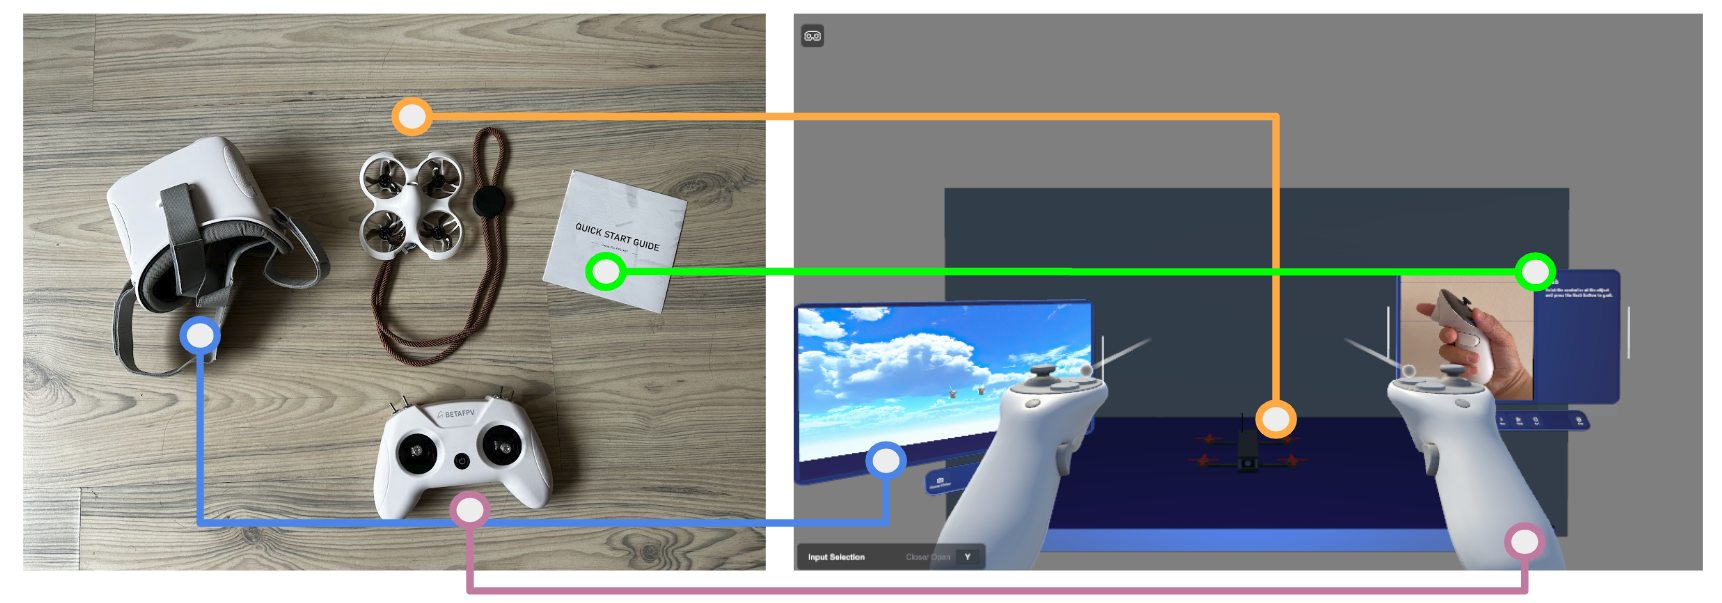
\includegraphics[width=0.8\linewidth]{img/stages/structure.png}
\end{figure}

\paragraph{Analysis}

Test play shows that player can understand the basic interaction of this system in third person view mode, but still can not understand direction well, especially when piloting through the DroneVision(FPV mode), the skydom designed for the quadcopter can not provide enough information for directions.

